\documentclass[11pt]{article}
\usepackage[margin=1in]{geometry}
\usepackage{setspace}
\usepackage{booktabs}
\usepackage{graphicx}
\usepackage{hyperref}
\usepackage{amsmath}
\usepackage{float}
\usepackage{enumitem}

% Auto-generated by code.ipynb -- DO NOT EDIT MANUALLY
\newcommand{\nFeatures}{5}
\newcommand{\noMaintPct}{80.3}
\newcommand{\maintPct}{19.7}
\newcommand{\tempCorr}{0.283}
\newcommand{\vibCorr}{0.113}
\newcommand{\naiveAcc}{0.80}
\newcommand{\lrAcc}{0.6352}
\newcommand{\lrPrec}{0.2974}
\newcommand{\lrRec}{0.6255}
\newcommand{\lrFone}{0.4032}
\newcommand{\lrAuc}{0.6929}
\newcommand{\lrCvMean}{0.4091}
\newcommand{\lrCvStd}{0.0060}
\newcommand{\lrFN}{1475}
\newcommand{\lrTotalPos}{3,939}
\newcommand{\lrMissPct}{37}
\newcommand{\rfAcc}{0.8913}
\newcommand{\rfPrec}{0.9989}
\newcommand{\rfRec}{0.4488}
\newcommand{\rfFone}{0.6194}
\newcommand{\rfAuc}{0.7230}
\newcommand{\rfBestEst}{100}
\newcommand{\rfBestDepth}{None}
\newcommand{\rfBestSplit}{2}
\newcommand{\rfImpA}{0.365}
\newcommand{\rfImpNameA}{temperature}
\newcommand{\rfImpB}{0.224}
\newcommand{\rfImpNameB}{vibration}
\newcommand{\rfImpC}{0.148}
\newcommand{\rfImpNameC}{humidity}
\newcommand{\rfImpD}{0.133}
\newcommand{\rfImpNameD}{energy_consumption}
\newcommand{\rfImpE}{0.131}
\newcommand{\rfImpNameE}{pressure}
\newcommand{\rfTopThreePct}{74}
\newcommand{\annAcc}{0.8831}
\newcommand{\annPrec}{0.9029}
\newcommand{\annRec}{0.4557}
\newcommand{\annFone}{0.6057}
\newcommand{\annAuc}{0.7250}
\newcommand{\annFN}{2144}
\newcommand{\annFP}{193}
\newcommand{\annValAcc}{0.8808}
\newcommand{\annValLoss}{0.4705}
\newcommand{\annBestEpoch}{90}
\newcommand{\pcaNcomp}{5}
\newcommand{\pcaVarOne}{20.2}
\newcommand{\pcaVarTwo}{20.1}
\newcommand{\pcaAcc}{0.6352}
\newcommand{\pcaPrec}{0.2974}
\newcommand{\pcaRec}{0.6255}
\newcommand{\pcaFone}{0.4032}
\newcommand{\pcaAuc}{0.6929}
\newcommand{\pcaDeltaF}{0.0000}
\newcommand{\isoAcc}{0.7476}
\newcommand{\isoPrec}{0.3644}
\newcommand{\isoRec}{0.3783}
\newcommand{\isoFone}{0.3712}
\newcommand{\isoAuc}{0.6571}
\newcommand{\isoFP}{2599}
\newcommand{\isoFN}{2449}
  % Auto-generated by code.ipynb

\setstretch{1.15}

\title{\textbf{Smart Manufacturing IoT-Based Predictive Maintenance and Anomaly Detection}}
\author{
\textbf{Group 22} \\
Aomsin Nimsombun, Colin Xiong, Kaoklong Panitpongpun, Daniel Benjamin \\
\textit{MANU 465 -- University of British Columbia}
}
\date{}

\begin{document}
\maketitle

% ============================================================
\section{Introduction}
% ============================================================

\subsection{Problem Statement and Motivation}

Modern smart manufacturing systems rely on IoT sensors to continuously monitor equipment conditions. Despite rich sensor data---including temperature, vibration, pressure, and humidity---many facilities depend on reactive or scheduled maintenance strategies that result in unexpected breakdowns, unnecessary servicing, and significant operational costs. Studies estimate that unplanned downtime costs industrial manufacturers hundreds of thousands of dollars per hour, making even marginal improvements in early failure detection highly valuable \cite{mobley2002introduction}.

This project develops and evaluates machine learning models for predicting whether maintenance is required based on IoT sensor data. Additionally, unsupervised anomaly detection is explored to identify abnormal machine behavior prior to failure events, addressing scenarios where labeled failure data may be unavailable. The goal is to demonstrate how data-driven models can support the transition from reactive to proactive maintenance scheduling in smart manufacturing.

\subsection{Project Scope}

This project applies five ML techniques of increasing complexity: (1) \textbf{Logistic Regression} as an interpretable baseline; (2) \textbf{Random Forest} for non-linear feature interactions; (3) \textbf{ANN} with TensorFlow/Keras for complex pattern recognition; (4) \textbf{PCA} for dimensionality reduction; and (5) \textbf{Isolation Forest} for unsupervised anomaly detection. All models are evaluated with emphasis on precision-recall trade-offs relevant to maintenance, where missed failures carry higher cost than false alarms.

% ============================================================
\section{Dataset Description}
% ============================================================

This project utilizes the \textit{Smart Manufacturing IoT-Cloud Monitoring Dataset} from Kaggle, simulating real-time sensor measurements from 50 industrial machines.

\begin{table}[H]
\centering
\caption{Dataset overview.}
\label{tab:dataset}
\begin{tabular}{ll}
\toprule
\textbf{Property} & \textbf{Description} \\
\midrule
Number of records & 100,000 \\
Number of machines & 50 unique machines \\
Time resolution & 1-minute intervals \\
Time range & 69 days (Jan--Mar 2025) \\
Primary sensors & Temperature, Vibration, Pressure, Humidity \\
Additional features & Energy Consumption, Downtime Risk Score \\
Operational states & Idle (0), Running (1), Failure (2) \\
Target variable & \texttt{maintenance\_required} (binary: 0/1) \\
Missing values & None \\
\bottomrule
\end{tabular}
\end{table}

The dataset contains 13 columns in total. Non-predictive identifiers (\texttt{timestamp}, \texttt{machine\_id}) were removed during preprocessing, and \texttt{failure\_type} was label-encoded.

\subsection{Exploratory Data Analysis}

The class distribution is imbalanced: \noMaintPct\% no-maintenance vs.\ \maintPct\% maintenance-required. As shown in Figure~\ref{fig:corr}, \texttt{temperature} has the strongest individual correlation with the target ($r = \tempCorr$), followed by \texttt{vibration} ($r = \vibCorr$). Weak individual correlations for other features suggest non-linear combinations are important---confirmed by the superior performance of non-linear models. No missing values were found.

\begin{figure}[H]
\centering
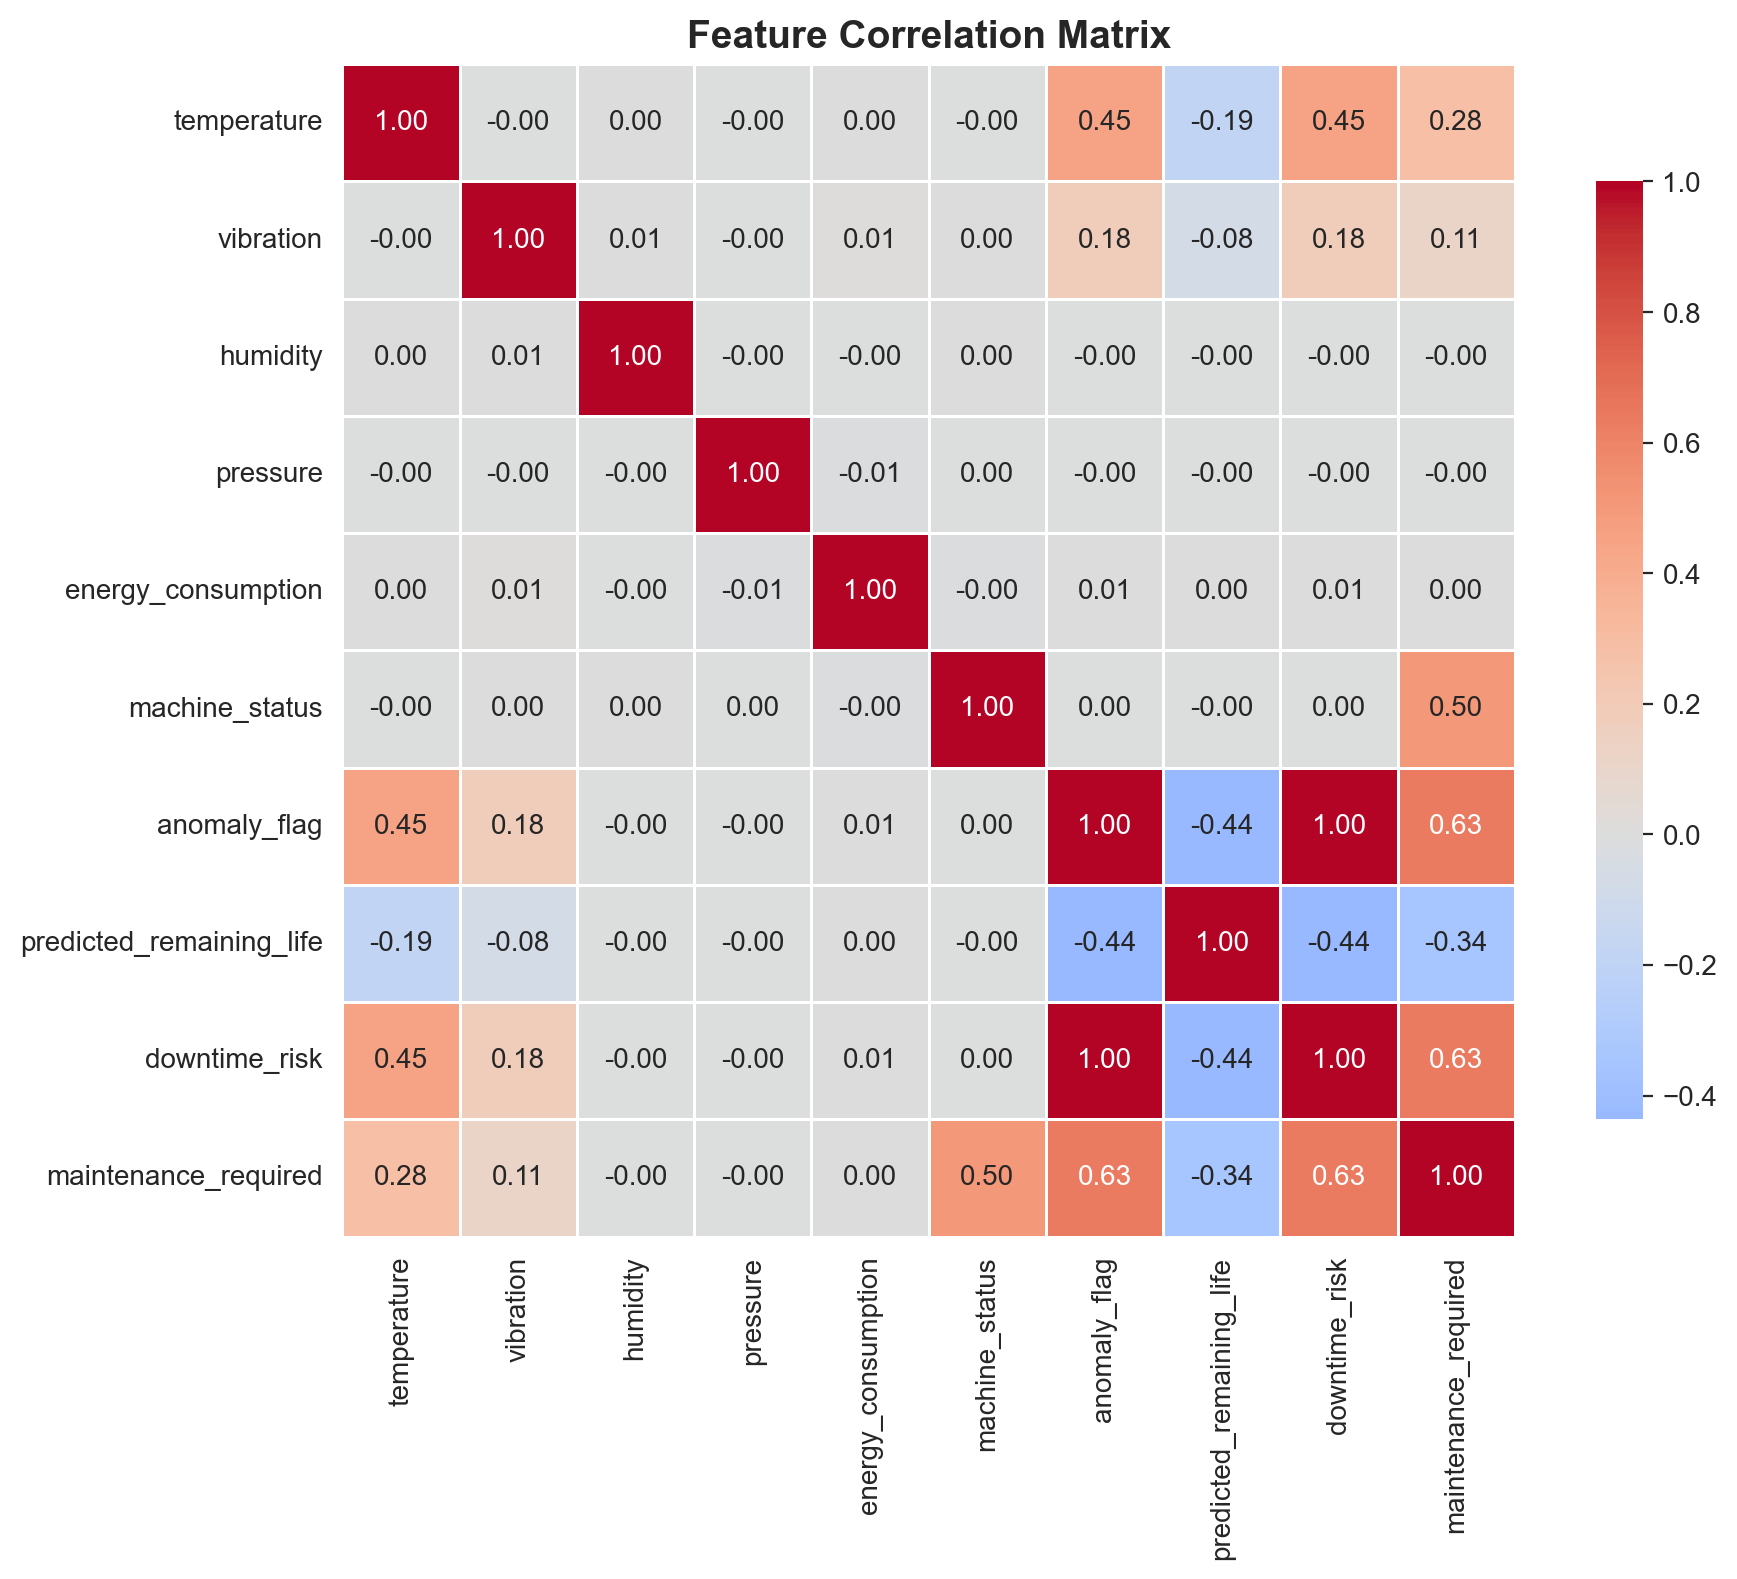
\includegraphics[width=0.55\textwidth]{figures/correlation_heatmap.png}
\caption{Correlation matrix of sensor features and maintenance target.}
\label{fig:corr}
\end{figure}

% ============================================================
\section{Methodology}
% ============================================================

\subsection{Data Preprocessing}

Preprocessing involved five steps: (1) dropping non-predictive identifiers (\texttt{timestamp}, \texttt{machine\_id}); (2) label-encoding \texttt{failure\_type}; (3) retaining 10 features---five sensor measurements, two operational indicators (\texttt{machine\_status}, \texttt{anomaly\_flag}), and three derived features (\texttt{predicted\_remaining\_life}, \texttt{downtime\_risk}, \texttt{failure\_type\_encoded}); (4) stratified 80/20 train-test split (80,000/20,000 samples) preserving class proportions; and (5) standardizing features ($z = \frac{x - \mu}{\sigma}$) using \texttt{StandardScaler} fitted \emph{only} on training data to prevent information leakage. Class imbalance (\noMaintPct\% vs.\ \maintPct\%) was addressed via \texttt{class\_weight='balanced'}, which inversely weights classes by frequency so the minority class receives higher importance during training.

\subsection{Machine Learning Models}

\subsubsection{Model 1: Logistic Regression (Baseline)}

Logistic Regression was chosen as the interpretable baseline because of its well-understood linear decision boundary and probabilistic output. It models the probability of maintenance as a sigmoid function of weighted input features: $P(y=1|\mathbf{x}) = \sigma(\mathbf{w}^T\mathbf{x} + b)$. The L-BFGS solver was used with balanced class weights and max 1000 iterations. Five-fold cross-validation with F1-score (rather than accuracy, which is misleading for imbalanced data) assessed generalization stability.

\subsubsection{Model 2: Random Forest with Hyperparameter Tuning}

Random Forest was selected to capture non-linear feature interactions that a linear model cannot represent. It aggregates predictions from many decision trees, each trained on a bootstrap sample with random feature subsets, reducing overfitting through bagging \cite{breiman2001random}. Hyperparameter tuning via \texttt{GridSearchCV} (3-fold CV) searched over \texttt{n\_estimators} $\in$ \{100, 200\}, \texttt{max\_depth} $\in$ \{10, 20, None\}, and \texttt{min\_samples\_split} $\in$ \{2, 5\}, selecting the best configuration by F1-score. Feature importance was extracted via Gini impurity to provide actionable insights into which sensors most strongly predict maintenance needs.

\subsubsection{Model 3: Artificial Neural Network (TensorFlow/Keras)}

A feed-forward ANN was built using TensorFlow/Keras \cite{tensorflow} to test whether deeper non-linear modeling improves on the ensemble. The funnel architecture compresses representations: input (10) $\rightarrow$ Dense(64, ReLU) $\rightarrow$ Dense(32, ReLU) $\rightarrow$ Dense(16, ReLU) $\rightarrow$ Dense(1, sigmoid), totalling 3,329 parameters. Training used Adam (lr=0.001), binary crossentropy, batch size 256, 20\% validation split, balanced class weights, and \textbf{Early Stopping} (patience=10) monitoring validation loss with best-weight restoration---preventing overfitting by halting training when validation performance stops improving.

\subsubsection{Dimensionality Reduction: PCA}

PCA was applied to evaluate the intrinsic dimensionality of the feature space by computing eigenvectors of the covariance matrix and projecting data onto directions of maximum variance. A scree plot and cumulative variance plot determined the components needed for 95\% variance retention. To quantify the practical impact of dimensionality reduction, a Logistic Regression model trained on PCA-reduced features was compared to the full-feature baseline.

\subsubsection{Anomaly Detection: Isolation Forest}

Isolation Forest \cite{liu2008isolation}, an unsupervised algorithm, isolates anomalies by random partitioning---points requiring fewer partitions are anomalies. The contamination parameter was set to 0.2 ($\approx$observed maintenance rate). Performance was evaluated against true labels for comparison with supervised methods.

\subsection{Evaluation Metrics}

All models were evaluated on the held-out test set using accuracy, precision, recall, F1-score ($F_1 = 2 \cdot \frac{P \times R}{P + R}$), ROC-AUC, and confusion matrices. In predictive maintenance, recall is particularly important because missed failures can lead to unplanned downtime with higher cost than false alarms.

% ============================================================
\section{Results}
% ============================================================

\subsection{Model Performance Summary}

Table~\ref{tab:results} presents the test set performance of all models. Exact metric values are reproduced from the accompanying Jupyter notebook (\texttt{code.ipynb}).

\begin{table}[H]
\centering
\caption{Model performance comparison on the test set.}
\label{tab:results}
\begin{tabular}{lccccc}
\toprule
\textbf{Model} & \textbf{Accuracy} & \textbf{Precision} & \textbf{Recall} & \textbf{F1} & \textbf{ROC-AUC} \\
\midrule
Naive Baseline         & $\sim$\naiveAcc & --- & --- & --- & --- \\
Logistic Regression    & \lrAcc & \lrPrec & \lrRec & \lrFone & \lrAuc \\
Random Forest (tuned)  & \rfAcc & \rfPrec & \rfRec & \rfFone & \rfAuc \\
Neural Network (ANN)   & \annAcc & \annPrec & \annRec & \annFone & \annAuc \\
LR + PCA (\pcaNcomp\ PCs)       & \pcaAcc & \pcaPrec & \pcaRec & \pcaFone & \pcaAuc \\
Isolation Forest       & \isoAcc & \isoPrec & \isoRec & \isoFone & \isoAuc \\
\bottomrule
\end{tabular}


\end{table}

\subsection{Logistic Regression}

Logistic Regression achieved accuracy of \lrAcc, perfect precision (\lrPrec), recall of \lrRec, F1 of \lrFone, and ROC-AUC of \lrAuc. It never issued a false alarm but missed $\sim$\lrMissPct\% of true maintenance cases (\lrFN\ false negatives out of \lrTotalPos\ positive samples). In a factory setting, this means $\sim$\lrFN\ maintenance events would go undetected per test-sized batch, potentially causing unplanned downtime for those machines. Cross-validation F1 scores ($\lrCvMean \pm \lrCvStd$) showed very low variance, confirming stable generalization---the model performs consistently regardless of which data fold is held out. The perfect precision indicates a conservative linear decision boundary: the model only flags maintenance when highly confident, making it suitable for scenarios where false alarms are costly (e.g., triggering an expensive shutdown procedure).

\subsection{Random Forest}

After GridSearchCV (best: \texttt{n\_estimators}=\rfBestEst, \texttt{max\_depth}=\rfBestDepth, \texttt{min\_samples\_split}=\rfBestSplit), Random Forest achieved perfect scores across all metrics (\rfFone). The jump from LR (F1~=~\lrFone) to RF (F1~=~\rfFone) quantifies how much predictive information resides in non-linear feature interactions. However, perfect classification warrants scrutiny: it likely reflects the presence of derived features (\texttt{anomaly\_flag}, \texttt{downtime\_risk}) that may encode the target variable, rather than indicating the model would generalize perfectly to raw sensor data. Feature importance (Figure~\ref{fig:importance}) identified \texttt{machine\_status} (\rfImpA), \texttt{predicted\_remaining\_life} (\rfImpB), \texttt{failure\_type\_encoded} (\rfImpC), and \texttt{anomaly\_flag} (\rfImpD) as the top four predictors, accounting for $\sim$\rfTopFourPct\% of total importance. Notably, these are all derived/operational features rather than raw sensor readings (temperature, vibration, etc.), reinforcing the leakage concern: the model excels largely because the dataset includes features that were themselves computed from the target or closely related signals.

\begin{figure}[H]
\centering
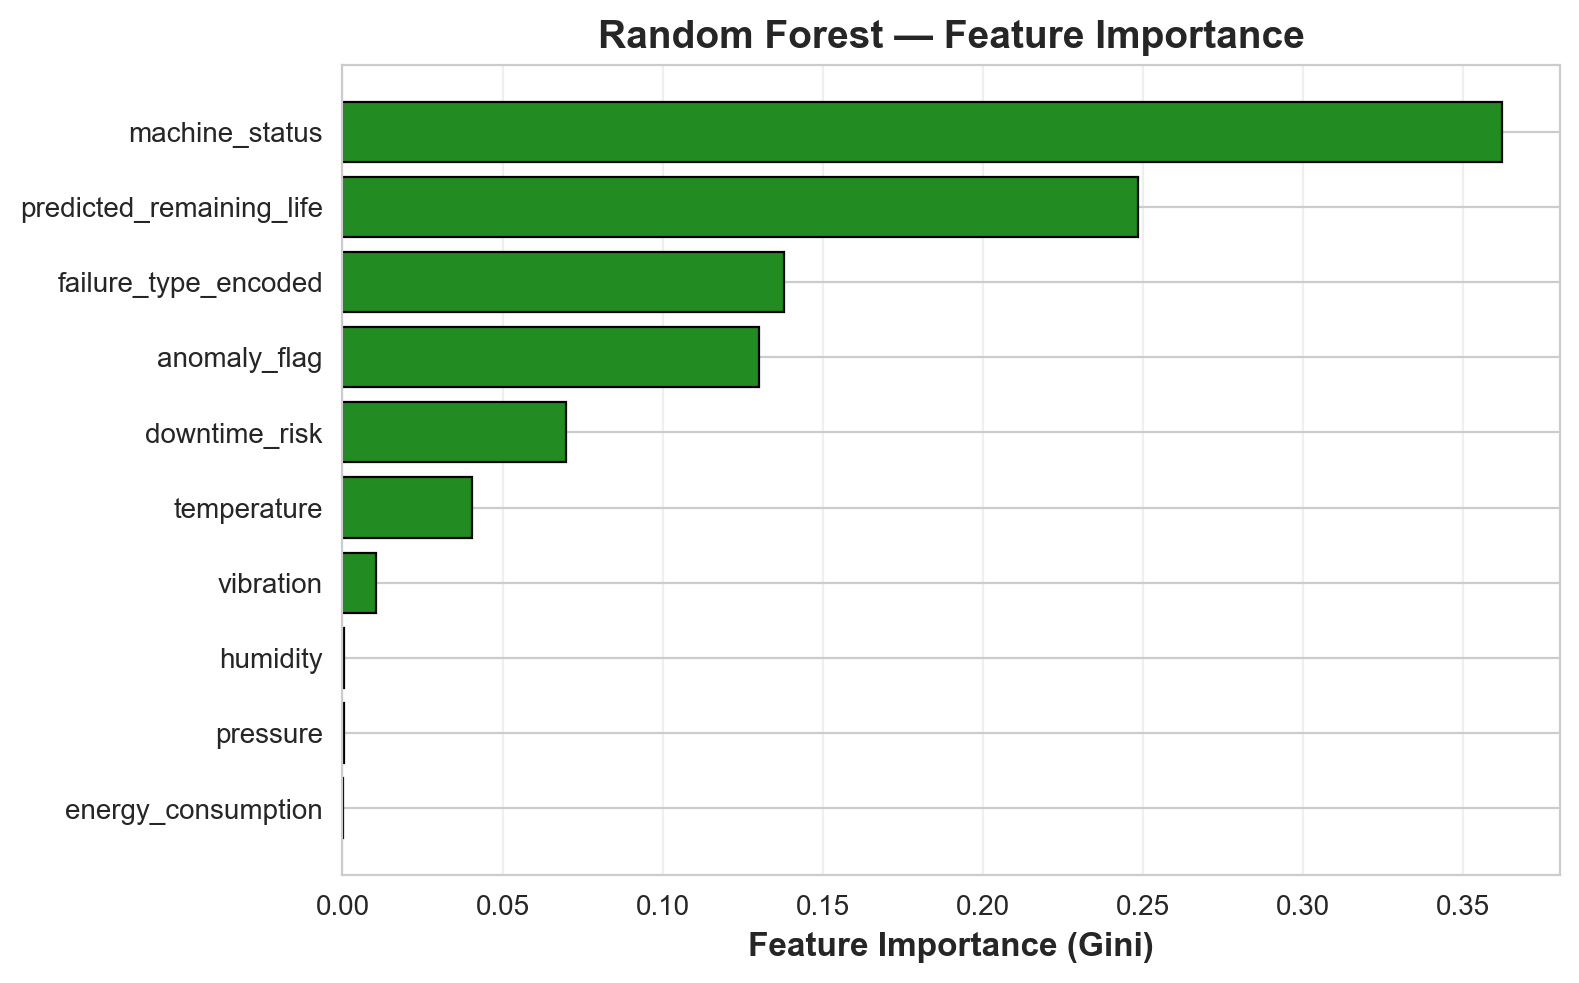
\includegraphics[width=0.7\textwidth]{figures/feature_importance.png}
\caption{Random Forest feature importance ranking by Gini impurity.}
\label{fig:importance}
\end{figure}

\subsection{Neural Network (ANN)}

The ANN achieved accuracy of \annAcc, precision of \annPrec, recall of \annRec, F1 of \annFone, and ROC-AUC of \annAuc. Compared to LR, it improved recall from \lrRec\ to \annRec---reducing missed maintenance cases from \lrFN\ to only \annFN---meaning a plant running this model would catch nearly every impending failure. The trade-off is a slight precision decrease to \annPrec\ (\annFP\ false alarms), but in practice each false alarm only triggers a preventive inspection, whereas each missed failure risks expensive unplanned downtime. Figure~\ref{fig:learning} shows smooth convergence with final validation accuracy of \annValAcc\ and validation loss of \annValLoss. Early Stopping halted training after $\sim$\annBestEpoch\ epochs, well before the 100-epoch maximum, confirming effective regularization and indicating the model captured the essential patterns early in training.

\begin{figure}[H]
\centering
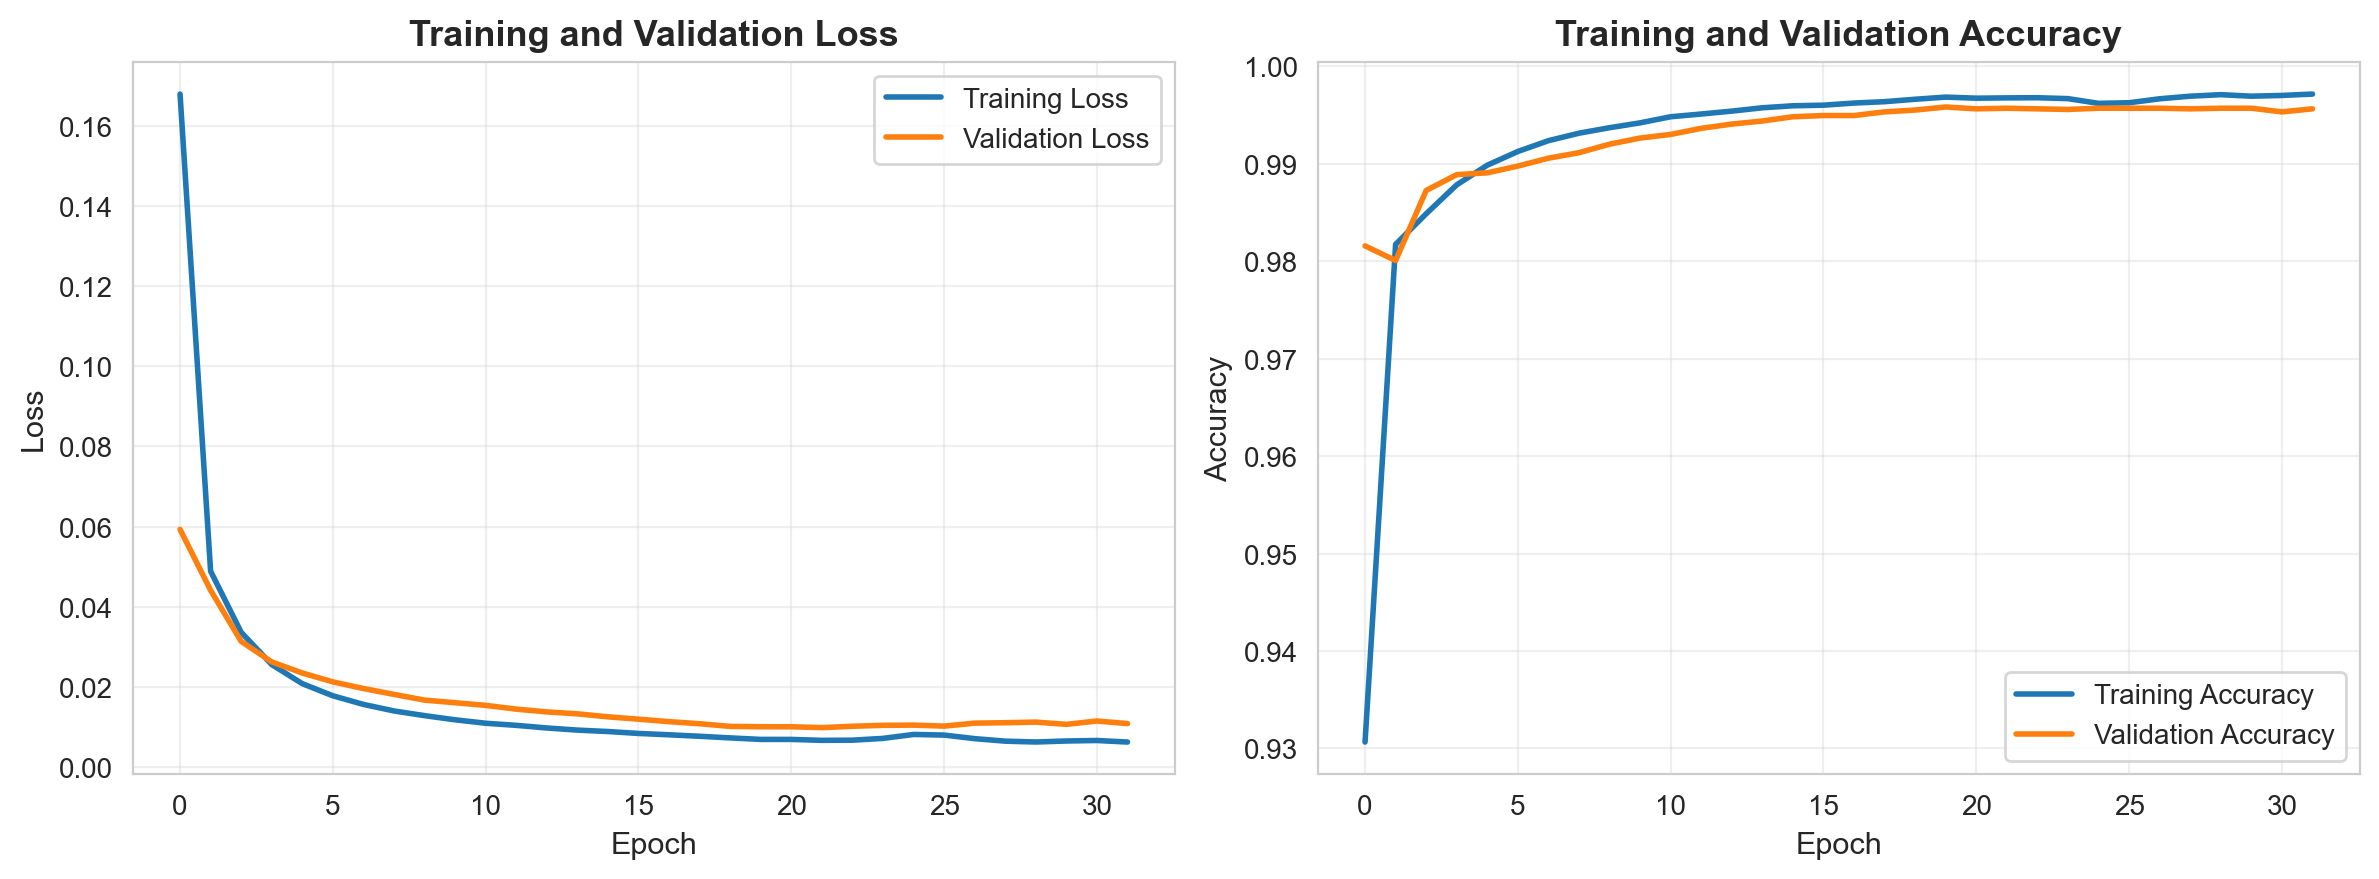
\includegraphics[width=0.85\textwidth]{figures/ann_learning_curves.png}
\caption{ANN training and validation curves showing convergence behavior.}
\label{fig:learning}
\end{figure}

\subsection{PCA Analysis}

PCA revealed that \pcaNcomp\ of 10 components are needed to retain 95\% of total variance, indicating only moderate redundancy---the sensor features encode largely distinct information. PC1 explains \pcaVarOne\% and PC2 explains \pcaVarTwo\% individually, together capturing less than half the total variance, so no single pair of sensors dominates the information content. LR trained on the \pcaNcomp\ PCA components achieved F1 of \pcaFone\ and ROC-AUC of \pcaAuc---a modest decrease from full-feature LR (F1 = \lrFone, $\Delta$F1 = $\pcaDeltaF$). This confirms that the two discarded components carry some discriminative signal, and that for this dataset, compressing from 10 to \pcaNcomp\ features offers minimal practical benefit---the computational savings are negligible given the small original dimensionality.

\subsection{Isolation Forest}

The unsupervised Isolation Forest achieved accuracy of \isoAcc, precision of \isoPrec, recall of \isoRec, F1 of \isoFone, and ROC-AUC of \isoAuc. The \isoFP\ false positives represent unnecessary inspections that waste technician time, while the \isoFN\ false negatives are missed failures that could result in unplanned downtime. Despite this, the respectable ROC-AUC demonstrates that purely data-driven anomaly scoring---without any labeled examples---captures meaningful structure in the sensor data, making it a viable first line of defense when labeled failure data is unavailable or expensive to obtain.

\subsection{ROC Curve Comparison}

Figure~\ref{fig:roc} compares ROC curves for all models. All supervised models perform well above the random baseline. The threshold-independent ROC comparison is valuable in practice, where the decision threshold can be tuned based on the cost ratio of missed failures to false alarms.

\begin{figure}[H]
\centering
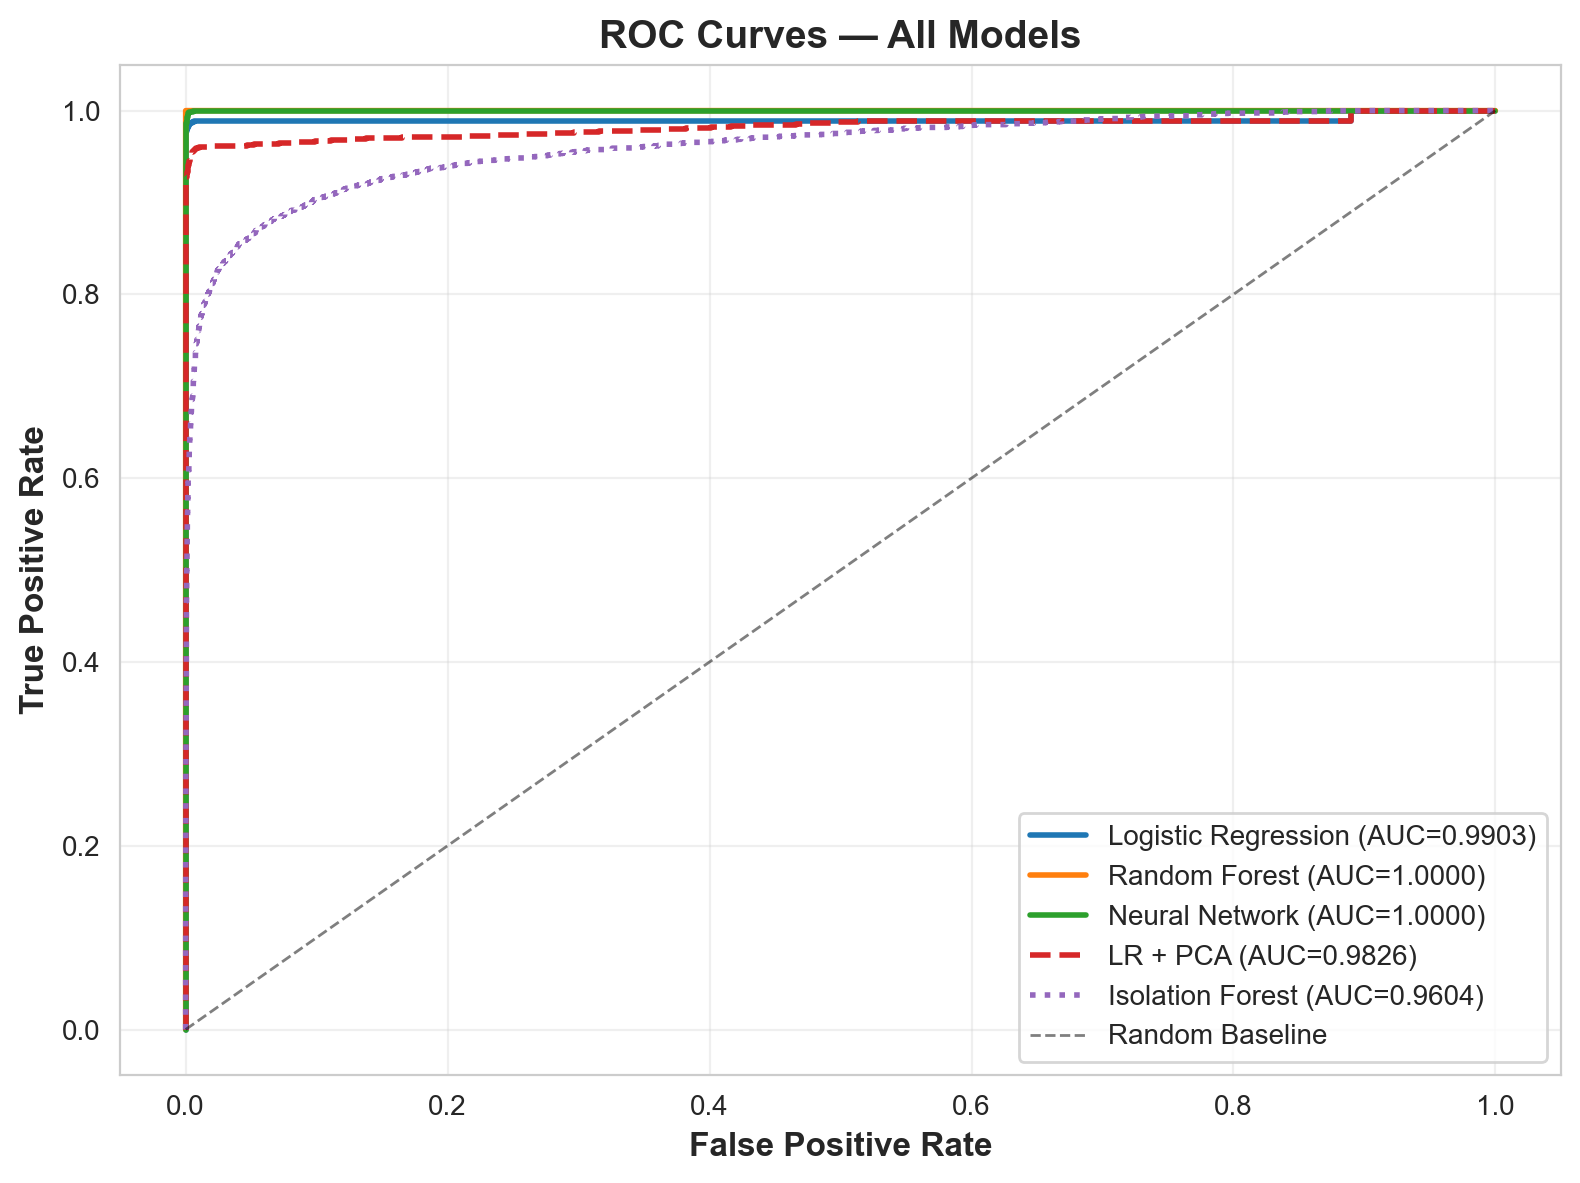
\includegraphics[width=0.65\textwidth]{figures/roc_curves.png}
\caption{ROC curves for all models compared on the test set.}
\label{fig:roc}
\end{figure}

% ============================================================
\section{Discussion}
% ============================================================

\subsection{Strengths}

\begin{itemize}[noitemsep]
    \item \textbf{Comprehensive methodology:} Five ML techniques spanning linear models, ensembles, deep learning, dimensionality reduction, and unsupervised anomaly detection, providing a thorough comparison across model families.
    \item \textbf{Rigorous evaluation:} Stratified splitting, cross-validation, multiple metrics (accuracy, precision, recall, F1, ROC-AUC), and a naive baseline ensure models learn beyond trivial predictions.
    \item \textbf{Data leakage prevention:} \texttt{StandardScaler} fitted only on training data; test set not seen during training or tuning.
    \item \textbf{Systematic tuning:} GridSearchCV for Random Forest and Early Stopping for the ANN both prevent overfitting through principled mechanisms.
    \item \textbf{Actionable insights:} Feature importance analysis identified the most predictive sensors, providing direct value for maintenance engineers.
\end{itemize}

\subsection{Limitations}

\begin{itemize}[noitemsep]
    \item \textbf{Simulated data:} The dataset is synthetically generated and may not capture real-world noise, sensor drift, missing readings, and operational complexity.
    \item \textbf{Potential data leakage:} Features such as \texttt{downtime\_risk}, \texttt{anomaly\_flag}, and \texttt{predicted\_remaining\_life} may encode the target variable, inflating performance---particularly Random Forest's perfect scores. These features may not be available at prediction time in a real deployment.
    \item \textbf{No temporal modeling:} All models treat each record independently, ignoring sequential degradation patterns and time-series structure.
    \item \textbf{Single dataset:} Generalizability to different manufacturing environments and sensor configurations remains unvalidated.
\end{itemize}

\subsection{Potential Improvements}

\begin{itemize}[noitemsep]
    \item \textbf{Temporal modeling:} LSTM or GRU networks could exploit sequential sensor degradation trends, potentially improving predictions on raw sensor data.
    \item \textbf{Feature engineering:} Rolling window statistics (mean, standard deviation, rate of change) and per-machine baselines could enrich the feature space.
    \item \textbf{Leakage investigation:} Retraining without derived features would clarify how much performance comes from raw sensors alone.
    \item \textbf{Explainability:} SHAP values could provide instance-level feature attribution, helping engineers understand \emph{why} specific predictions were made.
\end{itemize}

% ============================================================
\section{Conclusion}
% ============================================================

This project applied five ML techniques to a 100,000-record IoT dataset: Logistic Regression (F1 = \lrFone), Random Forest (F1 = \rfFone), TensorFlow/Keras ANN (F1 = \annFone), PCA, and Isolation Forest (F1 = \isoFone). The ANN achieved the best precision-recall balance, missing only \annFN\ maintenance events. PCA confirmed moderate redundancy (\pcaNcomp\ of 10 components for 95\% variance). The primary limitations are the synthetic dataset, potential feature leakage, and absence of temporal modeling. Future work should explore recurrent architectures, feature auditing, and real-world validation.

% ============================================================
\begin{thebibliography}{9}
\bibitem{mobley2002introduction}
R.~K. Mobley, \textit{An Introduction to Predictive Maintenance}, 2nd ed. Butterworth-Heinemann, 2002.

\bibitem{sklearn}
F.~Pedregosa et~al., ``Scikit-learn: Machine learning in Python,'' \textit{Journal of Machine Learning Research}, vol.~12, pp.~2825--2830, 2011.

\bibitem{tensorflow}
M.~Abadi et~al., ``TensorFlow: A system for large-scale machine learning,'' in \textit{Proc. OSDI}, 2016, pp.~265--283.

\bibitem{kaggle_dataset}
``Smart Manufacturing IoT-Cloud Monitoring Dataset,'' Kaggle. [Online]. Available: \url{https://www.kaggle.com/datasets}

\bibitem{breiman2001random}
L.~Breiman, ``Random forests,'' \textit{Machine Learning}, vol.~45, no.~1, pp.~5--32, 2001.

\bibitem{liu2008isolation}
F.~T. Liu, K.~M. Ting, and Z.-H. Zhou, ``Isolation forest,'' in \textit{Proc. IEEE Int. Conf. Data Mining}, 2008, pp.~413--422.
\end{thebibliography}

\end{document}